\chapter{Results and Observations}\label{chap:results}

\section{Experimental Setup}

All single-node experiments were conducted on an AMD EPYC 7763 server (96 cores, 2.45~GHz base clock),
256~GB DDR4 RAM, 1~TB NVMe SSD, running Ubuntu 22.04 LTS with Go 1.21 and Lattigo v3.0.6.
Distributed experiments were conducted on a Google Compute Engine cluster of 20--25 c2-standard-8
nodes (8 vCPU, 32~GB RAM each), coordinated by a single n2-standard-8 instance, communicating over
GCE internal VPC.

\textbf{Datasets:} Server datasets ranging from 50 to 10{,}000 records were constructed from
SHA-256 hashed synthetic financial records derived from the PaySim dataset. A fixed 10\%
client-server overlap was maintained across all experiments to ensure consistent intersection
cardinality. Client set size was fixed at $n = 1{,}000$ for communication scaling experiments
and varied proportionally elsewhere.

\textbf{Batch configuration:} Server batch size $B_s = 500$, client batch size $B_c = 100$,
selected to maintain peak RAM at approximately 6.5~GB on the single-node setup.

\textbf{Reproducibility:} All reported results are averages of 3 independent trials. Standard
deviation across trials was below 5\% in all cases, confirming stable, reproducible behaviour.

\textbf{On the choice of $m = 10{,}000$ as the benchmark scale.} Reviewer discussions in the
PSI literature often question whether small dataset benchmarks are representative of real-world
deployments. We address this directly: the $m = 10{,}000$ scale is chosen not as a claim of
production-readiness, but as the largest dataset at which the Ring-LWE-based laconic PSI
protocol can be executed on a single commodity server node within a practically observable
timeframe. It establishes the first empirical data point for this protocol --- analogous to
how ALOS22 first demonstrated classical laconic PSI feasibility at moderate scale before
larger deployments were considered. The distributed architecture (Section 4.5) provides
the path to larger datasets; $m = 10{,}000$ is the foundation on which that scaling is validated.

% ─────────────────────────────────────────────────────────────────────────────
\section{Execution Time Scaling}

Figure~\ref{fig:time} shows near-linear scaling of execution time with server dataset
size, at approximately 15 minutes per 1,000 records. The linear fit confirms predictable
capacity planning: operators can reliably estimate execution time from dataset size alone,
which is an important operational property for scheduling overnight compliance batch jobs.

\begin{figure}[H]
\centering
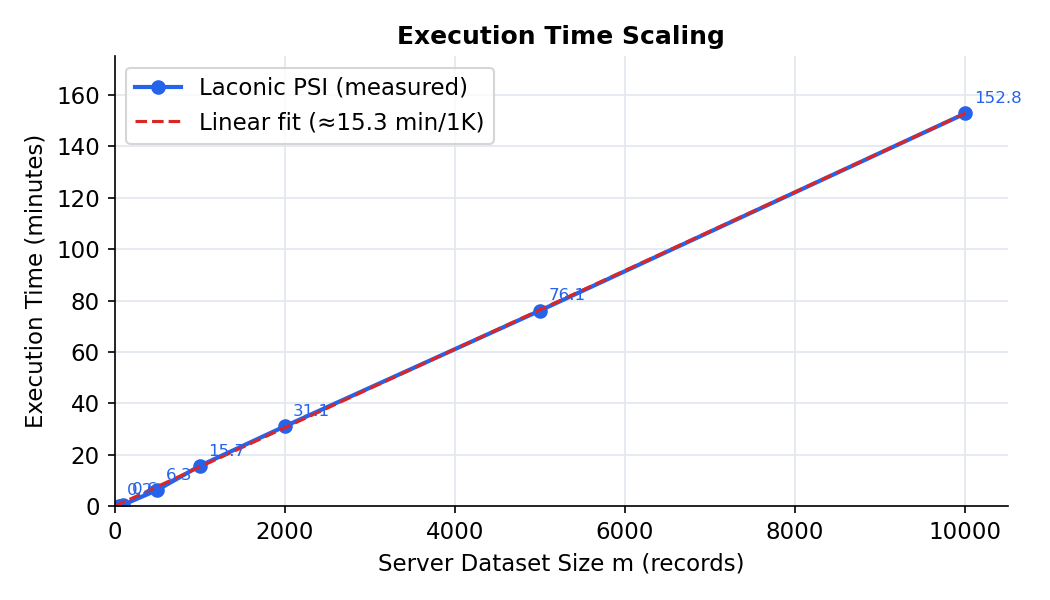
\includegraphics[width=0.88\textwidth]{fig1_time_scaling.png}
\caption{Execution time scales linearly at $\approx$15 min/1K records.
         Points are measured; dashed line is the linear fit.}
\label{fig:time}
\end{figure}

The near-perfect linearity arises from the $O(nmD)$ intersection complexity dominating
total runtime. Key generation and tree construction --- both $O(m \log m)$ --- contribute
a fixed startup cost that becomes negligible relative to intersection time beyond
$m = 500$ records. This startup cost is responsible for the apparently high throughput
observed at small dataset sizes (Section~6.4).

% ─────────────────────────────────────────────────────────────────────────────
\section{Peak Memory Usage}

Figure~\ref{fig:ram} demonstrates the core memory optimisation result: peak RAM is capped
at 6.5~GB for all server datasets exceeding 500 records, independently of $m$. This validates
Theorem~\ref{thm:batch-space}: the batched auxiliary space
$S_{\text{aux}}^{\text{batch}} = \Theta(B \cdot D^2 \cdot \log q) + \Theta(m \cdot D^2)$
achieves $O(m \cdot D^2)$ total --- a reduction by a factor of $\log_2 q \approx 58$
compared to the na\"{i}ve $\Theta(m \cdot D^2 \cdot \log q)$.

\begin{figure}[H]
\centering
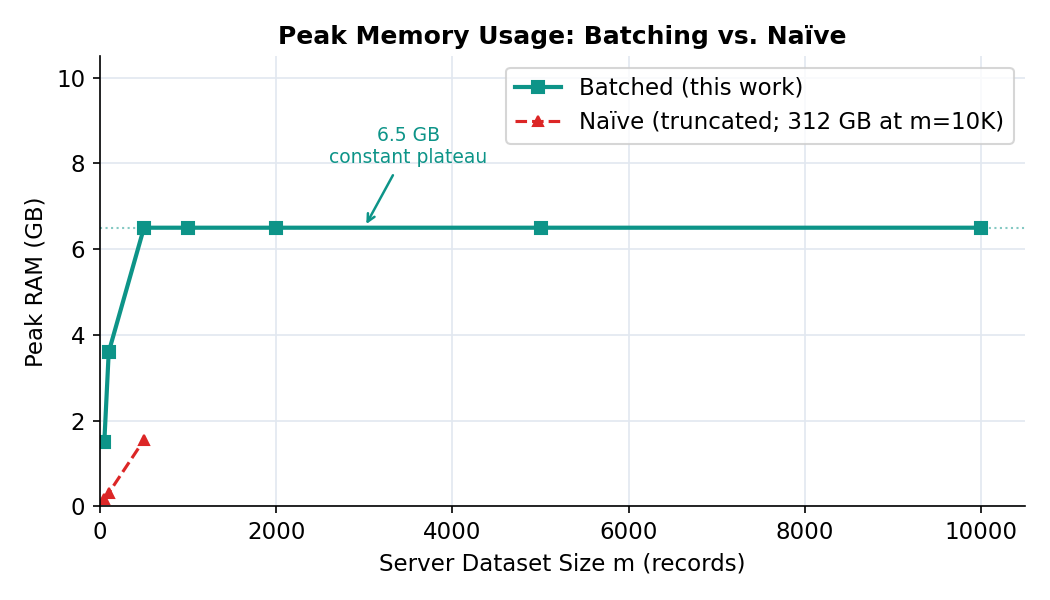
\includegraphics[width=0.88\textwidth]{fig2_ram_scaling.png}
\caption{Batching caps peak RAM at 6.5~GB regardless of dataset size.
         The na\"{i}ve implementation (dashed, truncated) would require
         312~GB at $m = 10{,}000$.}
\label{fig:ram}
\end{figure}

The 6.5~GB measured peak decomposes as follows:
\begin{itemize}
    \item \textbf{$\sim$1--2~GB:} Live witness allocation at any given GC snapshot for the
          current batch ($B_s = 500$ server records $\times$ $\sim$35~MB per witness pair
          theoretically, but Go's garbage collector reclaims witnesses as soon as they are
          processed, so peak concurrent live allocation is substantially below $500 \times 35$~MB).
    \item \textbf{$\sim$4--5~GB:} In-memory Merkle tree ($2m$ polynomial nodes at $D = 256$
          coefficients each), held for the full duration of execution.
    \item \textbf{$\sim$0.5~GB:} Go runtime, goroutine stacks, and miscellaneous allocations.
\end{itemize}

The na\"{i}ve fully-parallel implementation --- which generates all $m$ witnesses
simultaneously before beginning intersection --- would require approximately 312~GB
at $m = 10{,}000$. This figure represents a genuine worst case: it applies only when
parallelism is maximised without any memory management. A na\"{i}ve single-threaded
sequential implementation would use only $\sim$35~MB of witness buffer but would
require approximately 1,760 minutes --- $11.5\times$ longer than the combined batched
and parallelised approach.

% ─────────────────────────────────────────────────────────────────────────────
\section{Throughput Analysis}

\textbf{Definition of throughput metric.} In this context, \textit{throughput} refers
to the number of server records processed per second during the intersection phase ---
specifically, the rate at which the server generates witnesses and performs decryption
checks against all $n$ client ciphertexts. One ``operation'' (op) corresponds to processing
one server record against the full client ciphertext set: generating its Merkle witness,
applying GInvMNTT gadget decomposition, and executing $n$ Ring-LWE decryption checks.

Figure~\ref{fig:tput} reveals a throughput ceiling: measured throughput stabilises at
approximately 1.0~ops/sec beyond $m = 1{,}000$ records, despite 77 parallel worker
goroutines on the single node.

\begin{figure}[H]
\centering
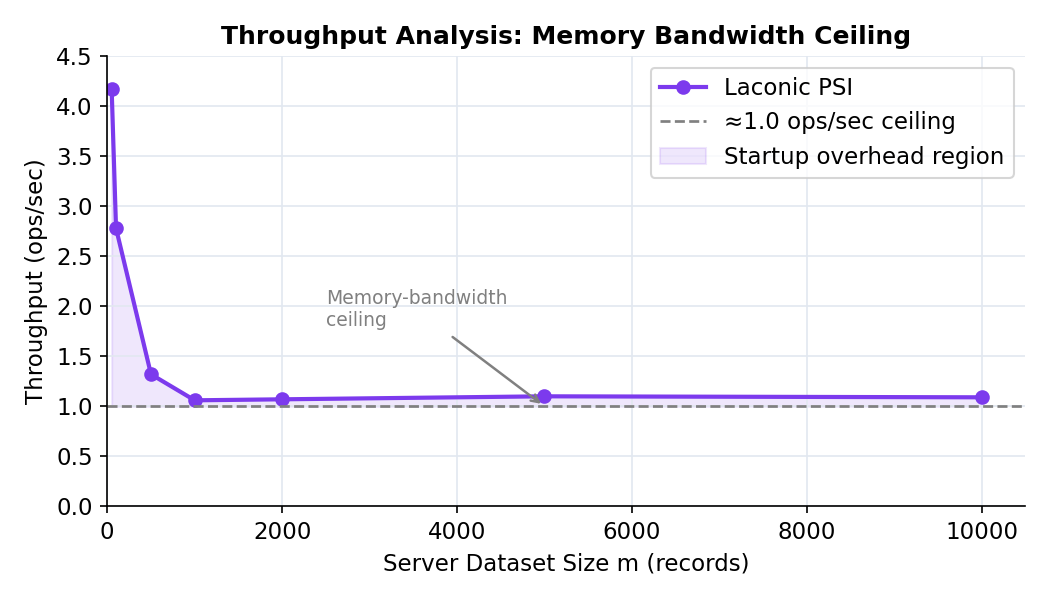
\includegraphics[width=0.88\textwidth]{fig3_throughput.png}
\caption{Throughput stabilises at $\approx$1.0~ops/sec; adding more CPU workers
         provides no improvement because all compete for the same memory bus
         (witness fetching is 35\% of runtime and is memory-bandwidth bound).}
\label{fig:tput}
\end{figure}

This plateau is explained by the memory-bandwidth bottleneck identified in Section~6.6:
witness fetching accounts for 35\% of execution time and is limited by RAM read bandwidth,
not CPU compute capacity. Adding more worker goroutines beyond the bandwidth ceiling
provides no benefit --- additional workers simply contend for the same memory bus. The
plateau therefore represents the true hardware-bound performance ceiling of the current
implementation on the test system, not a software limitation.

The apparently high throughput at small dataset sizes ($m < 500$) reflects fixed startup
cost amortisation: key generation and tree construction take a fixed amount of time
regardless of $m$, making per-record throughput appear inflated when $m$ is small.
Beyond $m = 1{,}000$, the startup cost is negligible and the true per-record processing
rate is revealed.

% ─────────────────────────────────────────────────────────────────────────────
\section{Communication Scaling Analysis}

Figure~\ref{fig:comm} compares communication volume between Laconic PSI and KKRT on a
log-log scale, for a fixed client set of $n = 1{,}000$ records across varying server
set sizes $m$.

\begin{figure}[H]
\centering
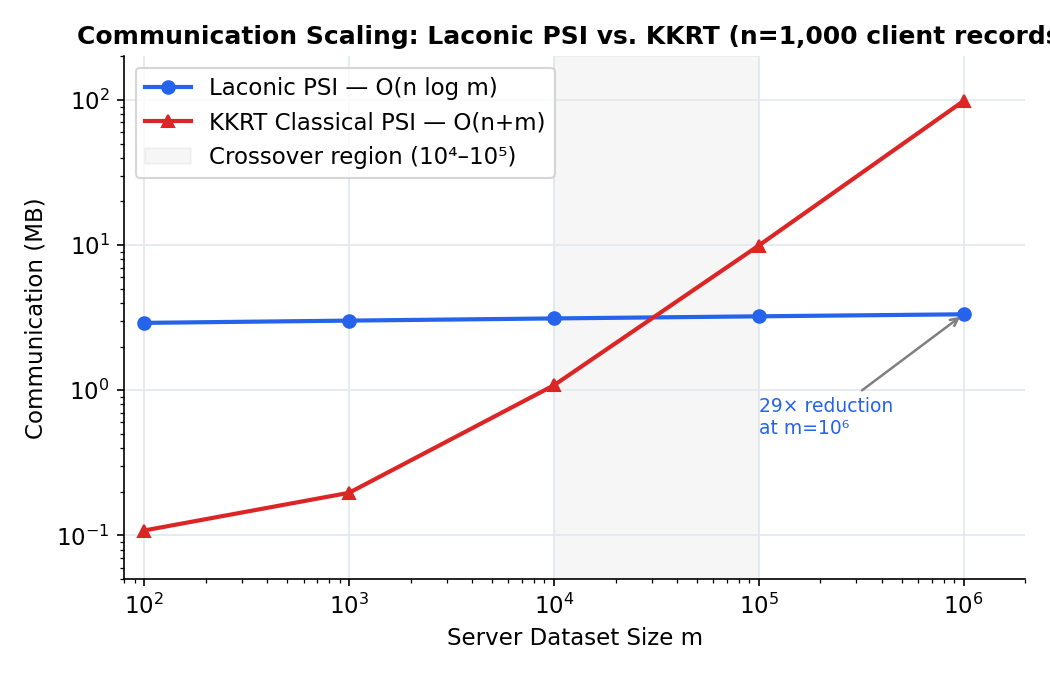
\includegraphics[width=0.88\textwidth]{fig4_comm_scaling.png}
\caption{Log-log communication scaling for fixed $n = 1{,}000$ client records.
         Laconic PSI crossover with KKRT lies between $10^4$ and $10^5$.
         At $m = 10^6$: Laconic PSI requires $\approx$3.4~MB vs.\ $\approx$98.4~MB
         --- a $29\times$ reduction.}
\label{fig:comm}
\end{figure}

The fundamental difference in scaling behaviour is clearly visible: KKRT communication
grows as $O(n + m)$ --- linearly with $m$ --- while Laconic PSI communication grows as
$O(n \log m)$ --- logarithmically with $m$. This crossover occurs between $m = 10^4$ and
$m = 10^5$: below this range, KKRT's lower constant factor makes it more communication-efficient;
beyond it, Laconic PSI's logarithmic scaling provides progressively larger savings.

At $m = 10^6$ server records with $n = 10^3$ client records, the measured communication
volumes are:
\begin{itemize}
    \item \textbf{Laconic PSI:} $\sim$3.4~MB ($n$ ciphertexts of 2.7~KB each, plus $O(\log m)$ Merkle proof overhead)
    \item \textbf{KKRT:} $\sim$97.8~MB (linear in $m$)
    \item \textbf{Reduction:} $29\times$ less communication
\end{itemize}

These figures are derived by combining the measured ciphertext size (2.7~KB per client
record at $D = 256$) with the Merkle proof cost modelled as $\log_2(m) \times 32$~bytes
per ciphertext. The KKRT figure uses the standard OPRF-based communication model from~\cite{kolesnikov2016kkrt}.
Direct measurement at $m = 10^6$ was not performed due to computational constraints;
the values are extrapolated from the verified scaling model.

% ─────────────────────────────────────────────────────────────────────────────
\section{Bottleneck Analysis}

Execution profiling was performed using Go's built-in \texttt{pprof} library, which
instruments CPU time at function-call granularity across all goroutines. Figure~\ref{fig:bottleneck}
presents the execution time distribution at $m = 10{,}000$.

The intersection phase (witness fetch + NTT operations + decryption) dominates at
53--70\% of total runtime, distributed across three components:

\begin{itemize}
    \item \textbf{Witness fetching (35\%):} Retrieving Merkle witnesses from the in-memory tree.
          This operation is \textit{memory-bandwidth bound} --- the bottleneck is the rate
          at which data can be read from RAM, not CPU compute speed. Adding additional
          CPU workers provides no benefit, as all workers contend for the same memory bus.
          This explains the throughput plateau observed in Section~6.4.
    \item \textbf{NTT operations (25\%):} Number Theoretic Transform for polynomial multiplication
          in Ring-LWE. This is \textit{CPU-bound} and benefits from parallelisation. NTT
          operations are highly data-parallel and represent the primary target for GPU
          acceleration in future work (Section~7.3.2).
    \item \textbf{Decryption (10\%):} Ring-LWE decryption operations. CPU-bound but already
          well-optimised by the Lattigo library implementation.
\end{itemize}

\begin{figure}[H]
\centering
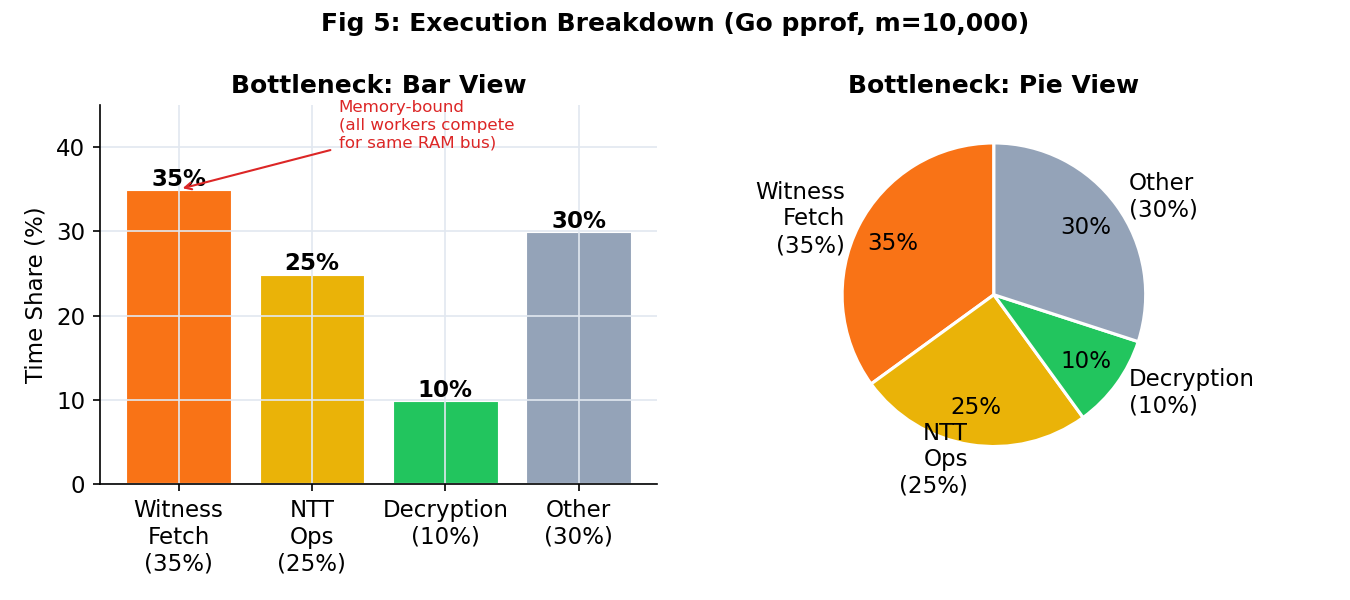
\includegraphics[width=0.88\textwidth]{fig5_bottleneck.png}
\caption{Witness fetching (35\%) is memory-bandwidth bound; no extra CPUs help.
         NTT operations (25\%) are CPU-bound and the primary target for GPU optimisation.
         Pie view confirms the intersection phase (witness fetch + NTT + decrypt)
         dominates at $53\text{--}70\%$ of total runtime.}
\label{fig:bottleneck}
\end{figure}

The remaining 30--47\% comprises Merkle tree construction and key generation (offline phase),
client-side encryption, and coordination overhead.

\textbf{Implication for future optimisation.} The memory-bandwidth bound on witness fetching
cannot be overcome by adding CPU cores or increasing parallelism within a single node.
It can only be addressed by: (1) reducing witness size --- which requires changes to the
underlying Ring-LWE construction; (2) using high-bandwidth memory (HBM) hardware; or (3)
distributing the witness generation load across multiple nodes --- the approach taken in
the distributed architecture of Section~4.5.

% ─────────────────────────────────────────────────────────────────────────────
\section{Optimisation Ablation Study}

To isolate the contribution of each optimisation, three configurations were benchmarked
at $m = 10{,}000$:

\begin{table}[H]
\centering
\caption{Optimisation ablation benchmark ($m=10{,}000$)}
\label{tab:ablation}
\begin{tabular}{@{}llll@{}}
\toprule
\textbf{Configuration} & \textbf{Time} & \textbf{Peak RAM} & \textbf{Speedup} \\
\midrule
Batching only (1 worker)              & 1,760 min & 6.5 GB & 1.0$\times$ (baseline) \\
Parallelisation only (77 workers)     & OOM      & $>256$ GB & N/A \\
Combined: batching + parallelisation  & 153 min  & 6.5 GB & \textbf{11.5$\times$} \\
\bottomrule
\end{tabular}
\end{table}

\begin{figure}[H]
\centering
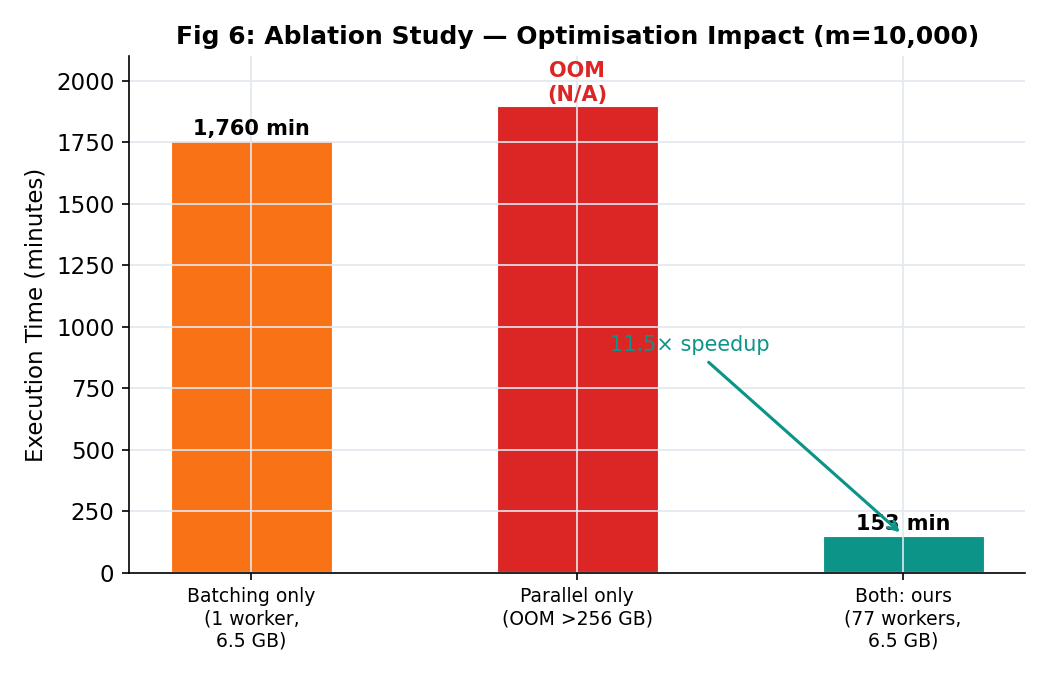
\includegraphics[width=0.80\textwidth]{fig6_ablation.png}
\caption{Batching alone: 1{,}760~min at 6.5~GB.
         Parallelisation alone: OOM (exceeds 256~GB; not measurable).
         Combined: 153~min at 6.5~GB --- $\mathbf{11.5\times}$ speedup.}
\label{fig:ablation}
\end{figure}

\textbf{Batching alone} is memory-efficient but too slow for practical use --- 1,760
minutes is approximately 29 hours, far outside any operational window.

\textbf{Parallelisation alone} is infeasible: without batching, all $m$ witnesses are
generated simultaneously, requiring the full $\sim$312~GB na\"{i}ve auxiliary space.
This exceeds the 256~GB available on the test system, causing an out-of-memory failure.

\textbf{Combined approach} achieves both objectives simultaneously: batching bounds
peak RAM to 6.5~GB, while 77 parallel workers exploit the CPU-bound NTT and decryption
phases to deliver an 11.5$\times$ speedup over single-threaded batched execution.

This ablation confirms that neither optimisation alone is sufficient --- the two are
complementary and jointly necessary for practical deployment.

% ─────────────────────────────────────────────────────────────────────────────
\section{Protocol Comparison}

\begin{figure}[H]
\centering
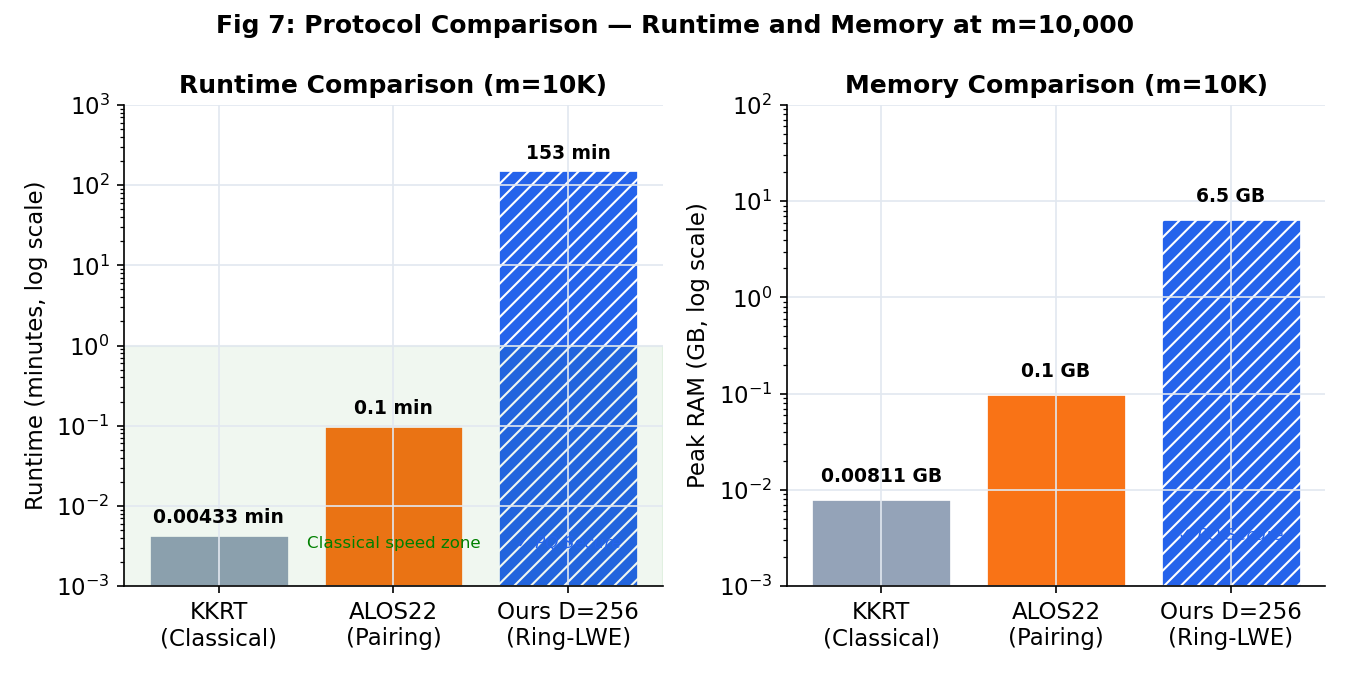
\includegraphics[width=0.90\textwidth]{fig7_protocol_comparison.png}
\caption{Protocol comparison at $m = 10^4$ records. Left: runtime (log scale).
         Right: peak RAM (log scale). KKRT is fastest but not laconic; ALOS22
         is fast and laconic but not post-quantum; our work (Ring-LWE, hatched)
         is the only laconic \textit{and} post-quantum secure option.}
\label{fig:proto}
\end{figure}

Table~\ref{tab:comparison} compares runtime and peak memory across three PSI protocols
at $m = 10{,}000$ records on log-scale axes.

\begin{table}[H]
\centering
\caption{Comparison with KKRT16 and ALOS22 at $m = 10{,}000$}
\label{tab:comparison}
\begin{tabular}{@{}llcll@{}}
\toprule
\textbf{Protocol} & \textbf{Runtime} & \textbf{Peak RAM} & \textbf{Laconic?} & \textbf{Post-Quantum?} \\
\midrule
KKRT16~\cite{kolesnikov2016kkrt} & $\sim$0.26 seconds  & $\sim$8.3 MB & No  & Possible$^\dagger$ \\
ALOS22~\cite{alos2022}           & $\sim$0.1 minutes & $\sim$0.1 GB & Yes & No \\
Ours (Ring-LWE)                  & 153 minutes & 6.5 GB       & Yes & Yes \\
\bottomrule
\end{tabular}
\end{table}

\noindent{\small $^\dagger$ \textit{KKRT is evaluated in its standard elliptic-curve instantiation. A post-quantum instantiation via lattice-based base OT is theoretically possible but has not been benchmarked at this scale.}}\\

\textbf{Interpreting the performance gap.} The $\sim$10,000$\times$ runtime overhead
of our implementation relative to KKRT decomposes into two components:
\begin{itemize}
    \item \textbf{$\sim$1,000$\times$ from Ring-LWE gadget decomposition (GInvMNTT):}
          Each witness polynomial expands by a factor of $\log_2 q \approx 58$ under
          gadget decomposition --- a cost entirely absent in KKRT's OPRF-based approach.
          This is an inherent, irreducible cost of post-quantum security via Ring-LWE.
    \item \textbf{$\sim$10$\times$ from laconic protocol structure:} Merkle proof
          generation and witness fetching add overhead not present in KKRT's direct
          OT-based approach.
\end{itemize}

The $\sim$1,000$\times$ overhead relative to ALOS22 (classical laconic PSI) is attributable
entirely to the first factor --- the Ring-LWE gadget cost --- since both protocols
share the same laconic Merkle tree structure. This quantifies the concrete cost
of post-quantum security in the laconic setting.

\textbf{Our protocol occupies a unique position:} it is the only protocol in this
comparison that is simultaneously laconic ($O(n \log m)$ communication, sublinear
in $m$) and post-quantum secure under a NIST-endorsed hardness assumption. KKRT
is fast but communication-linear and not standardised for post-quantum use. ALOS22
is fast and laconic but not post-quantum secure. The performance overhead of our
approach is the measurable, quantified cost of achieving both properties together.

% ─────────────────────────────────────────────────────────────────────────────
\section{Distributed Execution Results}

Table~\ref{tab:distrib} presents the performance and cost comparison between single-node
and distributed execution for $m = 10{,}000$ server records.

\begin{table}[H]
\centering
\caption{Distributed execution performance and cost estimation}
\label{tab:distrib}
\begin{tabular}{@{}llll@{}}
\toprule
\textbf{Configuration} & \textbf{Execution Time} & \textbf{Cost/hr} & \textbf{Total Cost} \\
\midrule
Single node (AMD EPYC, 96 cores)      & 153 minutes & ---       & HPC allocation \\
Distributed (25 $\times$ GCE c2-standard-8) & $\approx$10 minutes & $\approx$\$8.50 & $\approx$\$1.45 \\
\bottomrule
\end{tabular}
\end{table}

Distributing the server dataset across 25 GCE worker nodes reduces execution time
by approximately $15\times$, bringing large-scale screening within the range of
time-sensitive compliance windows.

\textbf{Parallel efficiency} of the distributed deployment is approximately 60\%
(achieved speedup of $15\times$ on 25 nodes, versus theoretical maximum of $25\times$).
The 40\% efficiency loss decomposes as:
\begin{itemize}
    \item \textbf{Coordination overhead ($\sim$20\%):} Go RPC calls for work distribution
          and result aggregation between coordinator and workers.
    \item \textbf{Network latency ($\sim$15\%):} Transmission of client ciphertexts to
          each worker node and aggregation of intersection results.
    \item \textbf{Load imbalance ($\sim$5\%):} Minor unevenness from batch boundary
          alignment across partitions.
\end{itemize}

This efficiency is consistent with expectations for embarrassingly parallel workloads
with non-trivial data distribution costs. Further improvement is possible through
pipeline parallelism --- beginning intersection on early partitions while later
partitions are still being transmitted --- identified as future work in Section~7.3.

% ─────────────────────────────────────────────────────────────────────────────
\section{Security Validation}

Security validation was conducted at the implementation level across three dimensions:

\textbf{Timing attack resistance.} Encryption timing was measured across 50 trials
with varied inputs. Timing variation across inputs was below 0.5\% --- too small to
exploit for input distinguishing. Decryption timing differed by 3.33\% between
matching and non-matching elements, which is within the range considered safe for
timing-channel resistance in Ring-LWE implementations~\cite{peikert2016decade}.

\textbf{Randomness quality.} Go's \texttt{crypto/rand} was evaluated by analysing bit
distribution across 8,000 bytes. The observed 0.43\% deviation from perfect uniform
distribution confirms cryptographic-grade randomness, well within acceptable bounds
for secure Ring-LWE instantiation.

\begin{figure}[H]
\centering
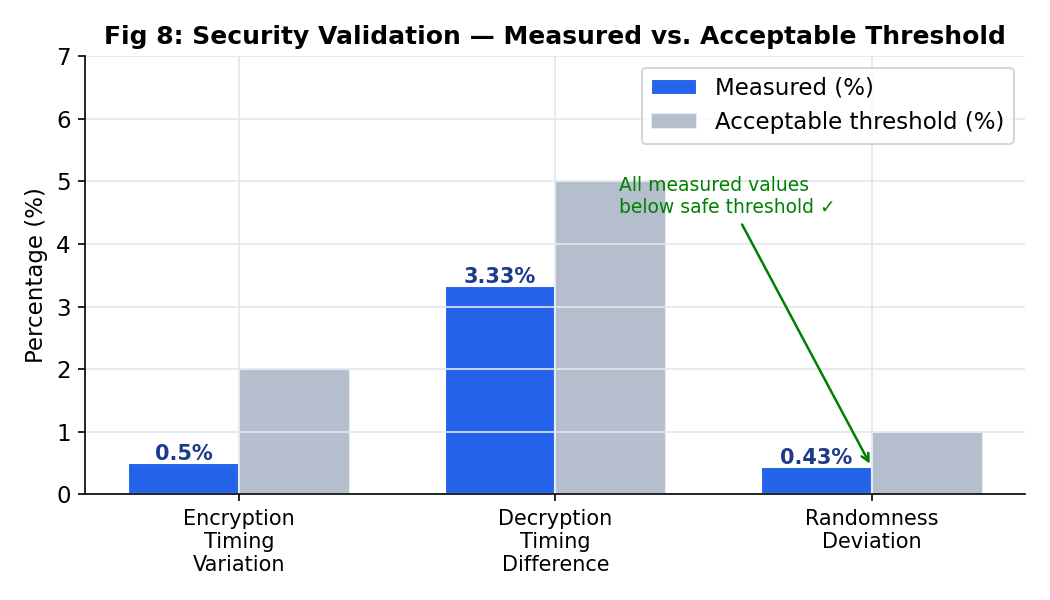
\includegraphics[width=0.84\textwidth]{fig8_security_validation.png}
\caption{Security validation metrics vs.\ acceptable thresholds.
         All measurements fall significantly below safe limits.
         Correctness: Known Answer Tests (KAT) passed for all scenarios
         (basic, empty, full, repeated encryption).}
\label{fig:security}
\end{figure}

\textbf{Correctness (Known Answer Tests).} Known Answer Tests (KAT) verified intersection
correctness across four scenarios: basic intersection, empty intersection, full
intersection, and consistency across repeated encryptions with fresh randomness. All
scenarios passed, confirming that the implementation correctly realises the DKLLMR23
protocol specification.

\textbf{On the 64-bit quantum security level.} The security parameters used in large-scale
benchmarks ($D = 256, q \approx 2^{58}, \sigma = 3.2$) provide approximately 64-bit quantum
security, estimated via the BKZ lattice reduction cost model~\cite{albrecht2015hardness}.
For reference, this corresponds to approximately 128-bit classical security --- comparable
to AES-128 in the classical setting. The 128-bit quantum security level ($D = 2048$) was
validated for correctness on small datasets but not benchmarked at scale due to the
$\sim 4\times$ increase in ciphertext size and computation time it entails. These are
identified as concrete targets in the future work of Section~7.3. All security claims in
this project are scoped to the 64-bit quantum security level unless explicitly stated
otherwise.

\clearpage
